The selection into preschool, as well as the selection into a particular type of preschool, might be determined by social, demographic, and economic characteristics of the family. We begin by presenting a linear probability model to predict the probability of selecting into (i) preschool or (ii) infant-toddler care and preschool based on background characteristics.

For an individual $i$, let $V_i$ indicate selection into preschool and $B_i$ indicate selection into both preschool and infant-toddler care.\footnote{There are too few individuals who selected only into infant-toddler care to consider that option as well.} Given a vector of binary characteristics $\mathbf{X}_i$, we perform the following regressions by city and cohort:

\begin{align}
	V_i &= \alpha_0 + \mathbf{X}_i\bm{\alpha} + \upsilon_i \label{eq:lpm-v} \\
	B_i &= \gamma_0 + \mathbf{X}_i\bm{\gamma} + \epsilon_i. \label{eq:lpm-b}
\end{align}

We combine Italian and non-Italian children into one cohort, but include an indicator for migrant in $\mathbf{X}$. Tables~\ref{tab:lpmRE} through \ref{tab:lpmPD} give the estimates of this model. These estimates reveal the percentage a particular characteristic contributes to the probability of enrolling in preschool (and infant-toddler care). 

\begin{sidewaystable}[H]
	\caption{Linear Probability Model, Reggio Emilia}\label{tab:lpmRE}
	\centering
	\footnotesize
		\begin{tabular}{lcccccccccc} \toprule
& \mc{2}{c}{Children} & \mc{2}{c}{Adolescents} & \mc{2}{c}{Adults 30s} &  \mc{2}{c}{Adults 40s} & \mc{2}{c}{Adults 50s} \\
\cmidrule(lr){2-3} \cmidrule(lr){4-5} \cmidrule(lr){6-7} \cmidrule(lr){8-9} \cmidrule(lr){10-11}
 & Preschool & Both & Preschool & Both & Preschool & Both & Preschool & Both & Preschool & Both \\ \midrule
One Sibling or More & 0.001 & 0.037 & 0.017 & -0.022 & 0.128** & 0.060 & -0.174** & -0.057 & 0.138 &  \\
 & (0.014) & (0.055) & (0.021) & (0.073) & (0.061) & (0.067) & (0.070) & (0.055) & (0.114) &  \\
Mother Max. Edu.: Middle Sch. & 0.027 & -0.035 & 0.026 & 0.254* & -0.040 & 0.252 & 0.289 & 0.347* & 0.643* &  \\
 & (0.029) & (0.115) & (0.037) & (0.130) & (0.422) & (0.464) & (0.256) & (0.201) & (0.338) &  \\
Mother Max. Edu.: High Sch. & 0.017 & 0.126** & 0.002 & 0.219*** & -0.148 & 0.128 & 0.182 & 0.320 & 0.615* &  \\
 & (0.015) & (0.062) & (0.024) & (0.084) & (0.437) & (0.481) & (0.247) & (0.194) & (0.348) & \\
Mother Max. Edu.: University & 0.020 & 0.269*** & 0.036 & 0.229** & -0.360 & 0.057 & 0.147 & 0.319 & 0.502 &  \\
 & (0.019) & (0.077) & (0.028) & (0.098) & (0.440) & (0.484) & (0.247) & (0.194) & (0.353) & \\
Father Max. Edu.: Middle Sch. & -0.041 & 0.077 & 0.012 & -0.148 & 0.002 & -0.751 & 0.246 & 0.013 & -0.299 &  \\
 & (0.028) & (0.111) & (0.035) & (0.123) & (0.436) & (0.479) & (0.231) & (0.181) & (0.333) &  \\
Father Max. Edu.: High Sch. & -0.003 & 0.014 & 0.005 & 0.028 & -0.013 & -0.697 & 0.201 & -0.229 & -0.600* &  \\
 & (0.014) & (0.057) & (0.021) & (0.073) & (0.395) & (0.434) & (0.223) & (0.175) & (0.345) & \\
Father Max. Edu.: University & 0.003 & 0.030 & -0.043 & 0.141 & 0.039 & -0.605 & 0.095 & -0.242 & -0.611* &  \\
 & (0.019) & (0.075) & (0.027) & (0.094) & (0.398) & (0.438) & (0.223) & (0.175) & (0.351) & \\
Caregiver is Religious & 0.057*** & -0.025 & -0.004 & -0.078 & -0.150*** & -0.120** & -0.100* & -0.059 & -0.058 &  \\
 & (0.016) & (0.066) & (0.020) & (0.071) & (0.050) & (0.055) & (0.052) & (0.041) & (0.072) &  \\
H. Income Above Median & -0.015 & -0.131*** & 0.023 & -0.005 &  &  &  &  &  &  \\
 & (0.012) & (0.050) & (0.018) & (0.061) &  &  &  &  &  &  \\
Caregiver Politics: Right of the Median & -0.003 & -0.064 & -0.017 & 0.021 &  &  &  &  &  &  \\
 & (0.014) & (0.055) & (0.017) & (0.060) &  &  &  &  &  &  \\
Low Birthweight & 0.011 & -0.001 & -0.008 & 0.007 &  &  &  &  &  &  \\
 & (0.028) & (0.111) & (0.042) & (0.148) &  &  &  &  &  &  \\
Premature Birth & 0.003 & 0.256** & -0.011 & -0.060 &  &  &  &  &  &  \\
 & (0.026) & (0.106) & (0.040) & (0.138) &  &  &  &  &  &  \\
Caregiver is a Migrant & 0.002 & -0.129 & -0.447*** & -0.070 &  &  &  &  &  &  \\
 & (0.026) & (0.104) & (0.073) & (0.256) &  &  &  &  &  &  \\
Non-Italian Child & -0.029 & -0.005 &  &  &  &  &  &  &  &  \\
 & (0.026) & (0.106) &  &  &  &  &  &  &  &  \\
Constant & 0.941*** & 0.561*** & 0.964*** & 0.429*** & 1.020* & 0.812 & 0.559*** & 0.085 & 0.069 &  \\
 & (0.024) & (0.095) & (0.029) & (0.102) & (0.591) & (0.650) & (0.167) & (0.131) & (0.359) &  \\
\midrule
$N$ enrolled & 415 & 242 & 293 & 170 & 223 & 69 & 205 & 41 & 53 & 0 \\
$N$ not enrolled & 6 & 179 & 7 & 130 & 57 & 211 & 80 & 244 & 147 & 200 \\
Total $N$ & 421 & 421 & 300 & 300 & 280 & 280 & 285 & 285 & 200 & 200 \\$R^2$ & 0.059 & 0.130 & 0.162 & 0.054 & 0.088 & 0.037 & 0.134 & 0.126 & 0.194 &  \\ \bottomrule
\end{tabular}

\end{sidewaystable}

\begin{sidewaystable}[H]
	\caption{Linear Probability Model, Parma}\label{tab:lpmPR}
	\centering
	\footnotesize
		\begin{tabular}{lcccccccccc} \toprule
& \mc{2}{c}{Children} & \mc{2}{c}{Adolescents} & \mc{2}{c}{Adults 30s} &  \mc{2}{c}{Adults 40s} & \mc{2}{c}{Adults 50s} \\
\cmidrule(lr){2-3} \cmidrule(lr){4-5} \cmidrule(lr){6-7} \cmidrule(lr){8-9} \cmidrule(lr){10-11}
 & Preschool & Both & Preschool & Both & Preschool & Both & Preschool & Both & Preschool & Both \\ \midrule
Mother Worked Full Time & 0.091*** & 0.420*** & 0.038* & 0.330*** & 0.152*** & 0.169*** & 0.242*** & 0.203*** & 0.421*** & 0.385*** \\
 & (0.027) & (0.076) & (0.022) & (0.088) & (0.057) & (0.062) & (0.071) & (0.044) & (0.083) & (0.058) \\
Mother Worked Part Time & 0.078*** & 0.423*** & 0.044* & 0.233** & -0.083 & 0.070 & 0.221** & 0.096* & 0.178 & 0.025 \\
 & (0.028) & (0.079) & (0.026) & (0.101) & (0.070) & (0.076) & (0.085) & (0.053) & (0.110) & (0.077) \\
Two Siblings or More & 0.026 & 0.109* & -0.033* & 0.041 & -0.152*** & -0.264*** & -0.236*** & -0.096** & -0.225** & -0.198*** \\
 & (0.023) & (0.064) & (0.020) & (0.077) & (0.052) & (0.057) & (0.068) & (0.043) & (0.102) & (0.071) \\
One Sibling or More & -0.015 & 0.048 & 0.025 & 0.077 & -0.044 & -0.119 & -0.052 & 0.002 & 0.015 & 0.068 \\
 & (0.021) & (0.059) & (0.019) & (0.077) & (0.077) & (0.083) & (0.112) & (0.070) & (0.160) & (0.112) \\
Mother Born in Province & -0.018 & -0.069 & 0.022 & -0.070 & -0.092* & -0.163*** & 0.107 & 0.057 & 0.027 & -0.034 \\
 & (0.022) & (0.061) & (0.018) & (0.070) & (0.053) & (0.058) & (0.073) & (0.046) & (0.104) & (0.073) \\
Mother Max. Edu.: Middle Sch. & -0.009 & 0.060 & -0.017 & 0.042 & 0.066 & 0.199 & 0.284 & 0.108 & 0.040 & 0.205 \\
 & (0.058) & (0.160) & (0.035) & (0.137) & (0.132) & (0.144) & (0.679) & (0.425) & (0.273) & (0.191) \\
Mother Max. Edu.: High Sch. & -0.008 & 0.053 & -0.044 & -0.118 & -0.048 & 0.100 & 0.153 & 0.064 & -0.197 & -0.050 \\
 & (0.031) & (0.086) & (0.028) & (0.110) & (0.066) & (0.072) & (0.688) & (0.431) & (0.283) & (0.199) \\
Mother Max. Edu.: University & -0.051 & 0.082 & -0.034 & -0.055 &  &  & 0.070 & 0.034 & -0.304 & -0.007 \\
 & (0.034) & (0.094) & (0.031) & (0.124) &  &  & (0.691) & (0.433) & (0.311) & (0.218) \\
Father Born in Province & 0.039* & -0.020 & 0.040** & -0.061 & -0.041 & -0.086 & -0.110 & -0.042 & 0.244*** & 0.071 \\
 & (0.022) & (0.060) & (0.019) & (0.076) & (0.058) & (0.063) & (0.085) & (0.053) & (0.089) & (0.063) \\
Father Max. Edu.: Middle Sch. & 0.033 & -0.032 & -0.011 & 0.129 &  &  & 0.259 & 0.028 & 0.298 & 0.121 \\
 & (0.044) & (0.121) & (0.035) & (0.140) &  &  & (0.486) & (0.304) & (0.241) & (0.169) \\
Father Max. Edu.: High Sch. & -0.015 & -0.064 & -0.004 & 0.073 & 0.157 & 0.048 & 0.287 & -0.075 & 0.282 & 0.004 \\
 & (0.026) & (0.071) & (0.024) & (0.094) & (0.120) & (0.131) & (0.491) & (0.308) & (0.244) & (0.171) \\
Father Max. Edu.: University & 0.010 & 0.009 & 0.005 & 0.112 & 0.178 & 0.070 & 0.541 & 0.006 & 0.549** & 0.039 \\
 & (0.028) & (0.078) & (0.027) & (0.108) & (0.124) & (0.135) & (0.495) & (0.310) & (0.269) & (0.188) \\
Caregiver is Religious & 0.008 & -0.083 & 0.033 & -0.071 & -0.016 & -0.006 & -0.074 & -0.015 & 0.034 & 0.111* \\
 & (0.028) & (0.078) & (0.025) & (0.098) & (0.055) & (0.060) & (0.074) & (0.046) & (0.087) & (0.061) \\
H. Income Above Median & 0.041** & -0.054 & 0.001 & -0.103 &  &  &  &  &  &  \\
 & (0.020) & (0.054) & (0.018) & (0.070) &  &  &  &  &  &  \\
Caregiver Politics: Right of the Median & -0.007 & -0.073 & -0.022 & -0.123* &  &  &  &  &  &  \\
 & (0.023) & (0.063) & (0.018) & (0.072) &  &  &  &  &  &  \\
Non-Italian Child & -0.051 & 0.045 &  &  &  &  &  &  &  &  \\
 & (0.074) & (0.191) &  &  &  &  &  &  &  &  \\
Low Birthweight & -0.004 & -0.338*** & -0.052 & -0.011 &  &  &  &  &  &  \\
 & (0.046) & (0.127) & (0.040) & (0.157) &  &  &  &  &  &  \\
Premature Birth & 0.038 & 0.176 & 0.009 & 0.074 &  &  &  &  &  &  \\
 & (0.042) & (0.117) & (0.033) & (0.131) &  &  &  &  &  &  \\
Constant & 0.902*** & 0.402*** & 0.923*** & 0.448*** & 0.837*** & 0.453** & 0.077 & 0.000 & -0.213 & -0.196 \\
 & (0.048) & (0.134) & (0.039) & (0.153) & (0.161) & (0.175) & (0.488) & (0.306) & (0.244) & (0.171) \\
\midrule
$N$ enrolled & 338 & 225 & 250 & 123 & 207 & 58 & 138 & 27 & 31 & 16 \\
$N$ not enrolled & 10 & 124 & 4 &131 & 44 & 193 & 116 & 227 & 72 & 87  \\
Total $N$ & 348 & 349 & 254 & 254 & 251 & 251 & 254 & 254 & 103 & 103 \\
$R^2$ & 0.089 & 0.151 & 0.092 & 0.124 & 0.144 & 0.175 & 0.164 & 0.144 & 0.433 & 0.554 \\ \bottomrule
\end{tabular}

\end{sidewaystable}

\begin{sidewaystable}[H]
	\caption{Linear Probability Model, Padova}\label{tab:lpmPD}
	\centering
	\footnotesize
		\begin{tabular}{lcccccccccc} \toprule
& \mc{2}{c}{Children} & \mc{2}{c}{Adolescents} & \mc{2}{c}{Adults 30s} &  \mc{2}{c}{Adults 40s} & \mc{2}{c}{Adults 50s} \\
\cmidrule(lr){2-3} \cmidrule(lr){4-5} \cmidrule(lr){6-7} \cmidrule(lr){8-9} \cmidrule(lr){10-11}
 & Preschool & Both & Preschool & Both & Preschool & Both & Preschool & Both & Preschool & Both \\ \midrule
Mother Worked Full Time when 6 & 0.003 & 0.258*** & 0.013 & 0.221*** & 0.034 & 0.132*** & 0.092 & 0.046 & 0.117 & 0.067 \\
 & (0.018) & (0.060) & (0.009) & (0.067) & (0.057) & (0.046) & (0.065) & (0.040) & (0.114) & (0.046) \\
Mother Worked Part Time when 6 & 0.000 & 0.170*** & 0.013 & 0.273*** & -0.057 & 0.061 & 0.062 & 0.188*** & -0.036 & 0.001 \\
 & (0.019) & (0.064) & (0.010) & (0.073) & (0.079) & (0.063) & (0.086) & (0.053) & (0.155) & (0.060) \\
Two Siblings or More & -0.010 & 0.158*** & 0.008 & 0.081 & -0.078 & -0.157*** & -0.082 & -0.111*** & 0.079 & 0.020 \\
 & (0.018) & (0.060) & (0.010) & (0.070) & (0.054) & (0.043) & (0.064) & (0.039) & (0.087) & (0.035) \\
One Sibling or More & 0.004 & 0.031 & -0.006 & 0.065 & -0.092 & 0.034 & -0.068 & 0.005 & 0.176 & 0.046 \\
 & (0.017) & (0.057) & (0.008) & (0.060) & (0.080) & (0.064) & (0.154) & (0.095) & (0.221) & (0.089) \\
Mother Born in Province & 0.031 & -0.170** & -0.000 & -0.072 & -0.000 & -0.044 & -0.049 & -0.039 & -0.220** & -0.060 \\
 & (0.020) & (0.067) & (0.009) & (0.064) & (0.056) & (0.045) & (0.060) & (0.037) & (0.104) & (0.042) \\
Mother Max. Edu.: Middle Sch. & 0.024 & -0.015 & -0.001 & -0.016 & -0.294 & -0.162 & -0.161 & 0.040 & 0.181 & -0.065 \\
 & (0.035) & (0.118) & (0.015) & (0.107) & (0.269) & (0.215) & (0.259) & (0.160) & (0.350) & (0.141) \\
Mother Max. Edu.: High Sch. & 0.022 & -0.085 & -0.005 & 0.105 & -0.208 & -0.175 & -0.252 & 0.108 & 0.430 & 0.056 \\
 & (0.020) & (0.068) & (0.011) & (0.076) & (0.246) & (0.197) & (0.254) & (0.156) & (0.377) & (0.152) \\
Mother Max. Edu.: University & 0.030 & 0.148* & 0.001 & 0.213** & -0.139 & -0.210 & -0.354 & 0.110 & 0.137 & -0.071 \\
 & (0.025) & (0.083) & (0.012) & (0.088) & (0.244) & (0.195) & (0.259) & (0.160) & (0.391) & (0.157) \\
Father Born in Province & -0.017 & -0.160** & -0.002 & -0.133** & -0.093 & -0.034 & -0.025 & -0.054 & -0.071 & 0.064 \\
 & (0.019) & (0.065) & (0.009) & (0.062) & (0.059) & (0.047) & (0.066) & (0.040) & (0.110) & (0.044) \\
Father Max. Edu.: Middle Sch. & 0.030 & -0.038 & -0.000 & 0.165 & 0.323 & -0.121 & -0.095 & -0.969*** & 0.099 & 0.070 \\
 & (0.034) & (0.115) & (0.015) & (0.108) & (0.232) & (0.185) & (0.324) & (0.200) & (0.309) & (0.124) \\
Father Max. Edu.: High Sch. & 0.038** & -0.038 & -0.006 & -0.014 & 0.106 & -0.151 & -0.093 & -1.032*** & 0.014 & 0.119 \\
 & (0.018) & (0.062) & (0.010) & (0.073) & (0.208) & (0.167) & (0.313) & (0.193) & (0.333) & (0.134) \\
Father Max. Edu.: University & 0.004 & -0.073 & -0.000 & -0.105 & 0.071 & -0.066 & -0.168 & -1.087*** & -0.060 & 0.035 \\
 & (0.023) & (0.078) & (0.012) & (0.083) & (0.205) & (0.164) & (0.316) & (0.195) & (0.336) & (0.135) \\
Caregiver is Religious & -0.017 & 0.072 & -0.003 & -0.065 & -0.058 & -0.047 & 0.114* & 0.045 & 0.044 & 0.045 \\
 & (0.021) & (0.069) & (0.008) & (0.060) & (0.056) & (0.045) & (0.067) & (0.041) & (0.101) & (0.040) \\
H. Income Above Median & 0.004 & -0.161*** & -0.005 & -0.026 &  &  &  &  &  &  \\
 & (0.017) & (0.057) & (0.008) & (0.056) &  &  &  &  &  &  \\
Caregiver Politics: Right of the Median & -0.008 & -0.035 & -0.003 & -0.011 &  &  &  &  &  &  \\
 & (0.019) & (0.064) & (0.008) & (0.057) &  &  &  &  &  &  \\
Non-Italian Child & -0.021 & -0.223 &  &  &  &  &  &  &  &  \\
 & (0.058) & (0.197) &  &  &  &  &  &  &  &  \\
Low Birthweight & 0.010 & 0.091 & -0.056*** & 0.027 &  &  &  &  &  &  \\
 & (0.034) & (0.114) & (0.019) & (0.131) &  &  &  &  &  &  \\
Premature Birth & 0.009 & 0.071 & -0.036** & 0.100 &  &  &  &  &  &  \\
 & (0.032) & (0.107) & (0.016) & (0.111) &  &  &  &  &  &  \\
Constant & 0.954*** & 0.544*** & 1.007*** & 0.121 & 1.099*** & 0.460** & 1.144*** & 1.104*** & 0.312 & -0.093 \\
 & (0.035) & (0.119) & (0.017) & (0.123) & (0.280) & (0.224) & (0.314) & (0.193) & (0.353) & (0.142) \\
\midrule
$N$ enrolled & 383 & 185 & 280 & 69 & 203 & 29 & 177 & 26 & 88 & 6 \\
$N$ not enrolled & 7 & 206 & 1 & 213 & 47 & 222 & 75 & 226 & 57 & 140 \\
Total $N$ & 390 & 391 & 281 & 282 & 250 & 251 & 252 & 252 & 145 & 146 \\
$R^2$ & 0.048 & 0.229 & 0.112 & 0.150 & 0.077 & 0.116 & 0.091 & 0.219 & 0.108 & 0.125 \\ \bottomrule
\end{tabular}

\end{sidewaystable}

The number of individuals in the different groups are listed at the bottom of the tables. In the younger cohorts, it is rare not to be enrolled in preschool, while in the older cohorts it is rare to be enrolled in both preschool and infant-toddler care. In Reggio Emilia, there are no individuals in the age-50 cohort enrolled in both infant-toddler care and preschool. For children and adolescents, it is more fruitful to examine the selection into both infant-toddler care and preschool, while for the adults the selection into preschool is more supported.

Higher education of the mothers is generally associated with higher enrollment in preschool and preschool and infant-toddler care, even across cohorts and cities. This is especially the case for younger cohorts in Reggio Emilia. Figures~\ref{fig:momEdu} and~\ref{fig:dadEdu} present the distribution of parental educational attainment for individuals from each combination of city, cohort, and preschool type. Figure~\ref{fig:momEdu} shows that within Reggio Emilia, mothers of individuals who did not attend preschool have proportionally higher levels of high school and university education than mothers of individuals who attended some form of preschool. This difference is more pronounced for the older cohorts, and statistically significant only for adults in their 50s (see Table~\ref{tab:lpmRE}). Figure~\ref{fig:dadEdu} shows that a similar pattern persists when examining father's education. A clear pattern does not emerge when we compare parental educational attainment between individuals who attended different types of preschool in Reggio Emilia. This suggests that parental education might have played a larger role in the initial decision of sending an individual to preschool, as compared to the subsequent decision of choosing a particular type of preschool. Figures~\ref{fig:momEdu} and~\ref{fig:dadEdu} include analogous graphs for Parma and Padova.

Figure~\ref{fig:parentsEdu} examines the difference of educational attainment between mothers and fathers for individuals from each city-cohort combination. Each column represents the total proportion of individuals in each city-cohort combination whose fathers are more educated than mothers. Each column is further broken down into sections that calculate this proportion conditional on different levels of father's education. The figures show that total inequality in educational attainment is largest in Padova and smallest in Reggio Emilia, and that this ranking of total inequality is consistent across the three adult cohorts. Furthermore, for the older cohorts, the level of inequality is substantially larger in Padova compared to Reggio Emilia and Parma. Padova is similar to the other two cities for the cohorts younger than the age-40 cohort. 


\begin{figure}[!htb]
	\begin{minipage}{1\textwidth}
	\centering
	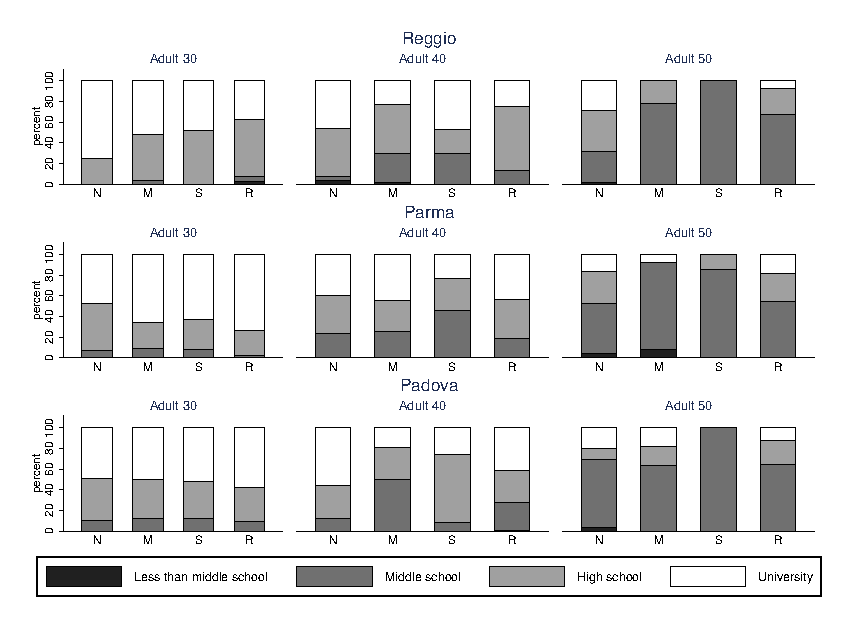
\includegraphics[scale=1.2]{../../output/image/bar_momEdu}
	\caption{Mother's Educational Attainment by City, Cohort and Preschool Type}
	\label{fig:momEdu}
	\footnotetext{Note:  \textbf{(1)} Definiteion of bar labels: N = Not attended; M = Municipal; S = State; R = Religious. \textbf{(2)} Each bar presents the distribution of mothers' educational attainment for individuals in each city-cohort-preschool type combination. }
	\end{minipage}
\end{figure}

\begin{figure}[!htb]
	\begin{minipage}{1\textwidth}
	\centering
	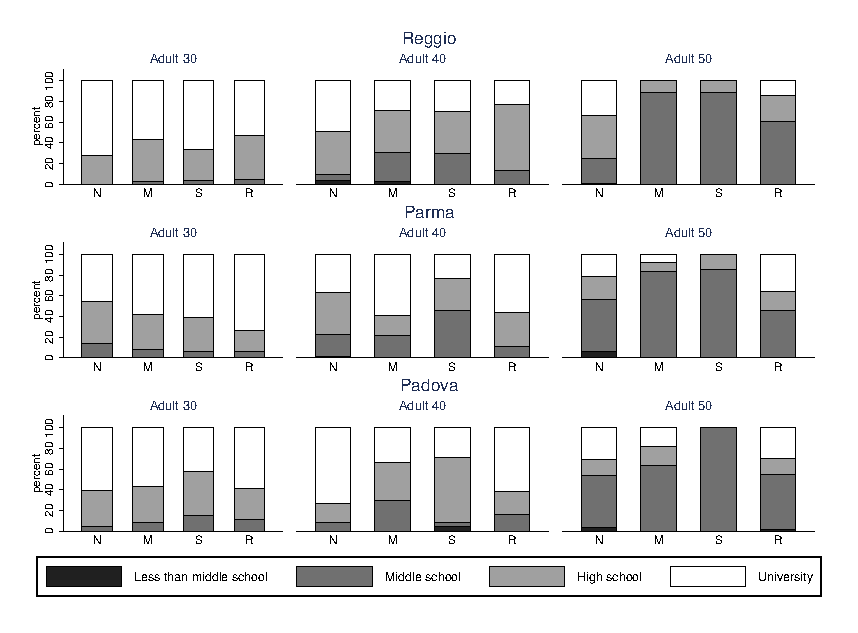
\includegraphics[scale=1.2]{../../output/image/bar_dadEdu}
	\caption{Father's Education Attainment by City, Cohort and Preschool Type}
	\label{fig:dadEdu}
	\footnotetext{Note:  \textbf{(1)} Definition of bar labels: N = Not attended; M = Municipal; S = State; R = Religious. \textbf{(2)} Each bar presents the distribution of fathers' educational attainment for individuals in each city-cohort-preschool type combination. }
	\end{minipage}
\end{figure}

\begin{figure}[!htb]
	\begin{minipage}{.9\textwidth}
	\centering
	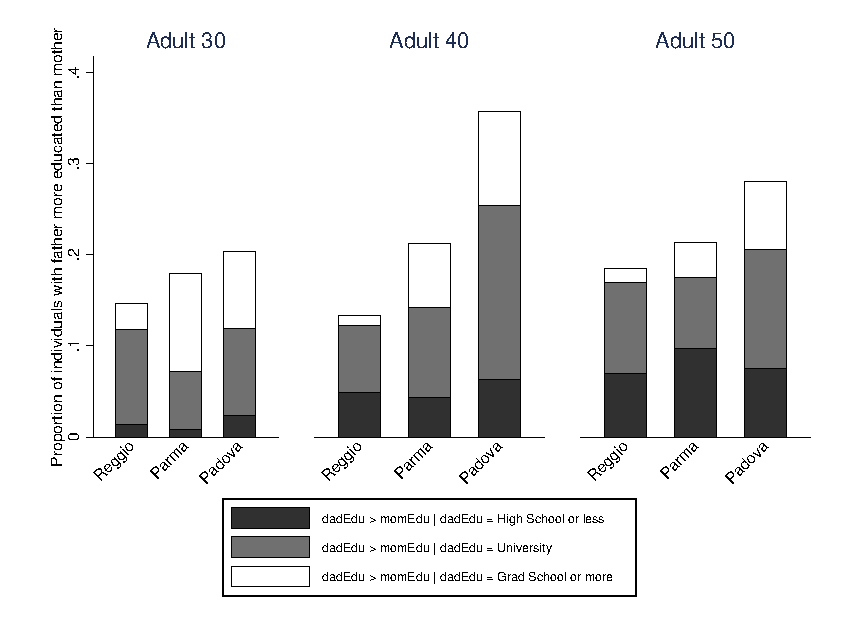
\includegraphics[scale=1]{../../output/image/bar_parentsEduCompare}
	\caption{Proportion of Individuals with Fathers who are More Educated than Mothers by City and Cohort}
	\label{fig:parentsEdu}
	\footnotetext{\noindent Note: Each column represents the proportion of individuals within each city-cohort combination whose fathers were more educated than their mothers.}
	\end{minipage}
\end{figure}

Although the above correlations help us understand some of the potential characteristics determining selection, one omitted variable is the mother's employment status. For the younger cohorts, measures for parental characteristics are measured after the birth of the children. Thus, including these characteristics in the the naive linear probability model above can produce biased results. We discuss several potential instruments for enrollment in preschool (and infant-toddler care). The second stage then uses this estimated first stage and a vector of controls to predict mother's working status and education.

One potential instrument is a measure of distance to the nearest preschool or infant-toddler center. We construct two indicators to be used in an IV regression for preschool and preschool and infant-toddler care separately. The first is an indicator that is 1 when the family lives closer than the sample median to the nearest preschool. The second is the analogous indicator for the nearest infant-toddler care. Table~\ref{tab:dist-center} shows a preliminary first stage to predict enrollment in preschool and both preschool and infant-toddler care. 

\begin{table}[H]
\begin{center}
\caption{First Stage in Reggio Emilia, Distance to Nearest Center} \label{tab:dist-center}
\scalebox{0.7}{
\begin{tabular}{lcccccccccc} \toprule
& \mc{2}{c}{Children} & \mc{2}{c}{Adolescents} & \mc{2}{c}{Adults 30s} & \mc{2}{c}{Adults 40s} & \mc{2}{c}{Adults 50s} \\
\cmidrule(lr){2-3} \cmidrule(lr){4-5} \cmidrule(lr){6-7} \cmidrule(lr){8-9} \cmidrule(lr){10-11}
 & Preschool & Both & Preschool & Both & Preschool & Both & Preschool & Both & Preschool & Both \\
 \midrule
 &  &  &  &  &  &  &  &  &  &  \\
 Close to Preschool & -0.016 &  & -0.008 &  & 0.046 &  & 0.047 &  & 0.049 &  \\
 & (0.011) &  & (0.017) &  & (0.046) &  & (0.049) &  & (0.058) &  \\
Close to Infant-toddler Care &  & 0.040 &  & -0.016 &  & 0.074 &  & -0.015 &  &  \\
 &  & (0.048) &  & (0.059) &  & (0.051) &  & (0.040) &  &  \\
Constant & 0.957*** & 0.650*** & 0.975*** & 0.409*** & 1.075* & 0.797 & 0.160 & 0.014 & -0.255 &  \\
 & (0.025) & (0.107) & (0.032) & (0.114) & (0.589) & (0.643) & (0.173) & (0.144) & (0.389) & \\
\midrule
Observations & 409 & 409 & 299 & 299 & 280 & 280 & 285 & 285 & 199 & 199 \\
$R^2$ & 0.080 & 0.152 & 0.093 & 0.081 & 0.136 & 0.102 & 0.247 & 0.145 & 0.227 &  \\ \bottomrule
\end{tabular}
}
\end{center}
\raggedright Note: This table shows the first stage using distance to the nearest center. Control variables are omitted in this table, although they are used in the regressions that produce these estimates. There are no individuals in the age-50 cohort who attended both preschool and infant-toddler care.
\end{table}


